\documentclass[12pt]{exam}
\usepackage[phy]{template-for-exam}
\usepackage{multicol}
\usepackage{tikz}
\usetikzlibrary{arrows.meta}
\tikzset{f/.append style={-{Stealth[length=3mm,width=2mm]}}}

\title{Net Force Examples}
\author{Rohrbach}
\date{\today}

\newcommand{\hforce}[2]
{
  \draw[f] (a) -- ++(#1, 0) 
        node[anchor=south] {#2};
}
\newcommand{\vforce}[2]
{
  \draw[f] (a) -- ++(0, #1) 
        node[anchor=west] {#2};
}

\begin{document}
\maketitle

\begin{questions}
  
  \question 
    In each of the free-body diagrams below, calculate the 
    {\bf magnitude} and {\bf direction} of the net force 
    and draw it.
  

    \begin{center}  
      \begin{tikzpicture}[scale=0.8]
        \newcommand{\createFBD}[1]
          {
            \filldraw (a) circle [radius=0.15];
            \path (a) node {} 
              + (0,-3.5) node {
                $F_{NET}=\fillin[][3em]$ N, \fillin[][4em]
              }
              + (-3,2.5) node {#1} ;
          }

        \begin{scope}
          \node (a) at (-5,4) {};
          \createFBD{(a)}
          \vforce{ 2}{\SI{18}{\newton}};
          \vforce{-2}{\SI{18}{\newton}};

        \end{scope}

        \begin{scope}
          \node (a) at (4,4) {};
          \createFBD{(b)}
          \vforce{  2  }{\SI{40}{\newton}};
          \vforce{-1.25}{\SI{24}{\newton}};
        \end{scope}

        \begin{scope}
          \node (a) at (-5,-4) {};
          \createFBD{(c)}
          \vforce{ 2}{\SI{5}{\newton}};
          \vforce{-2}{\SI{5}{\newton}};
          \hforce{ 3}{\SI{7}{\newton}};
          \hforce{-3}{\SI{7}{\newton}};
        \end{scope}

        \begin{scope}
          \node (a) at (4,-4) {};
          \createFBD{(d)}
          \vforce{  2 }{\SI{17}{\newton}};
          \vforce{ -2 }{\SI{17}{\newton}};
          \hforce{  3 }{\SI{32}{\newton}};
          \hforce{-1.5}{\SI{14}{\newton}};
        \end{scope}
      \end{tikzpicture}
    \end{center}


    \hrule 

        
  \question 
    In each of the free-body diagrams below, the net force 
    is given, but one or more of the applied forces is 
    missing.  Find the missing forces.

    \begin{EnvUplevel}
      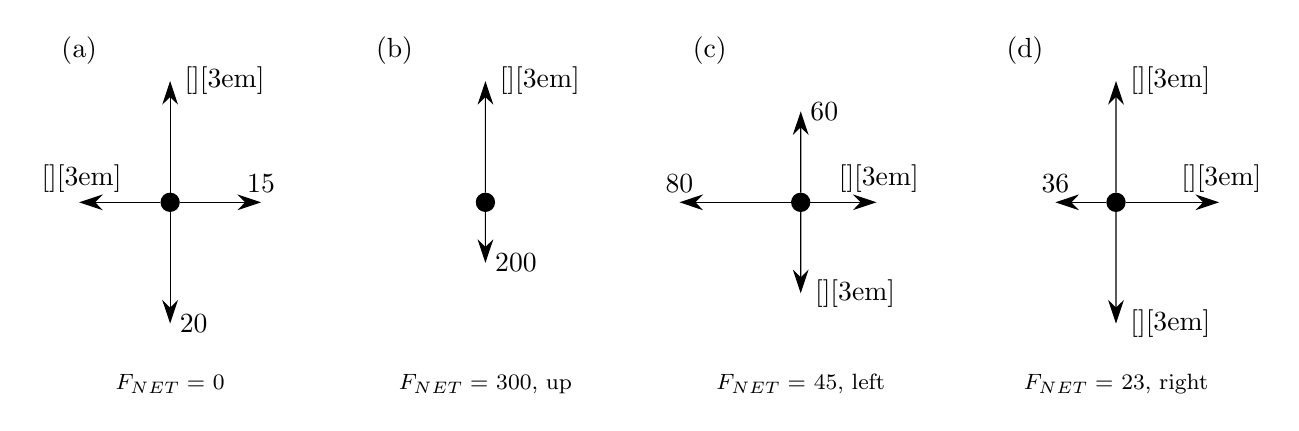
\begin{tikzpicture}[scale=0.77]
        \def\sep{5.2}

        \newcommand{\createFBD}[2]
          {
            \filldraw (a) circle [radius=0.15];
            \path (a) node {} 
              + (0,-3) node {\footnotesize
                $F_{NET}=$ #2
              }
              + (-1.5,2.5) node {#1} ;
          }
        \newcommand{\forceblank}
          {\,\fillin[][3em]\SI{}{\newton}}


        \begin{scope}
          \node (a) at (0,0) {};
          \createFBD{(a)}{\SI{0}{\newton}}
          \vforce{  2 }{\forceblank}
          \vforce{ -2 }{\SI{20}{\newton}}
          \hforce{ 1.5}{\SI{15}{\newton}}
          \hforce{-1.5}{\forceblank}
        \end{scope}

        \begin{scope}
          \node (a) at (\sep,0) {};
          \vforce{  2 }{\forceblank}
          \vforce{ -1 }{\SI{200}{\newton}}
          \createFBD{(b)}{\SI{300}{\newton}, up}
        \end{scope}

        \begin{scope}
          \node (a) at (2*\sep,0) {};
          \createFBD{(c)}{\SI{45}{\newton}, left}
          \vforce{  1.5 }{\SI{60}{\newton}}
          \vforce{ -1.5 }{\forceblank}
          \hforce{1.25}{\forceblank}
          \hforce{ -2 }{\SI{80}{\newton}}
        \end{scope}

        \begin{scope}
          \node (a) at (3*\sep,0) {};
          \createFBD{(d)}{\SI{23}{\newton}, right}
          \vforce{  2 }{\forceblank}
          \vforce{ -2 }{\forceblank}
          \hforce{ 1.7}{\forceblank}
          \hforce{ -1 }{\SI{36}{\newton}}
        \end{scope}

      \end{tikzpicture}
    \end{EnvUplevel}

  \pagebreak

  \question
    What is the acceleration of a 1500-kg car that
    experiences a net force of 970 N?
    \vs

  \question
    Fill in the blanks in each of the situations depicted 
    below.  Draw the net force.

    \begin{center}  
      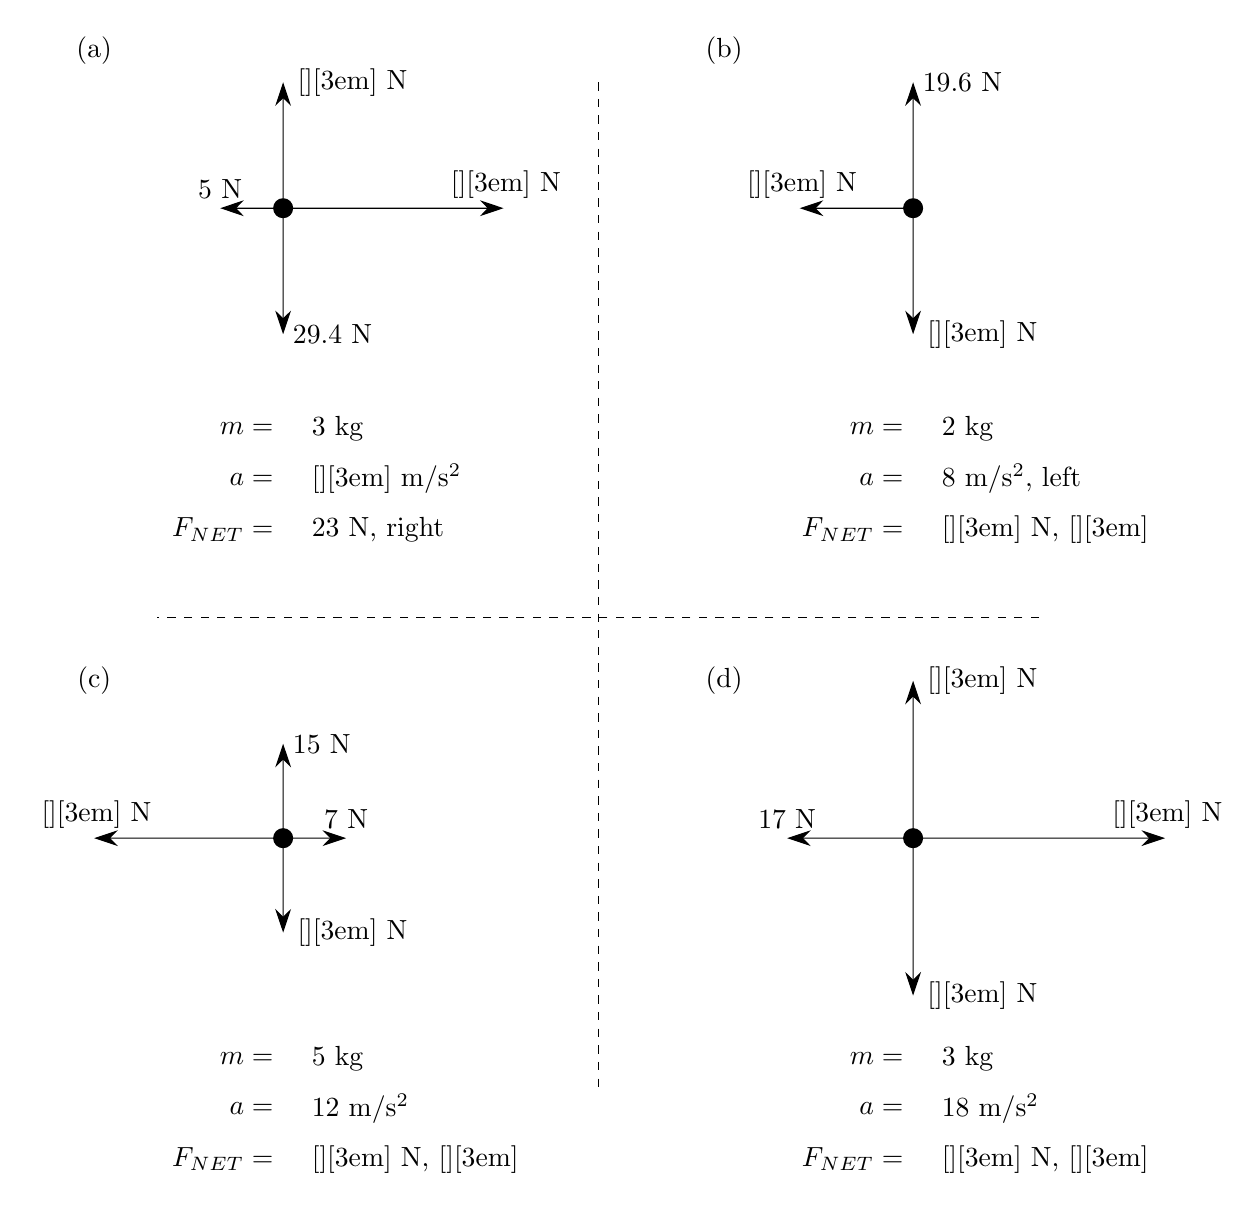
\begin{tikzpicture}[scale=0.8]
        \newcommand{\createFBD}[4]
          {
            \filldraw (a) circle [radius=0.15];
            \path (a) node {} 
              + (-3,2.5) node {#1}
              ++ ( 0,-3.5) node[anchor=east] {$m=$}
              ++ ( .3,  0) node[anchor=west] {#2}
              ++ (-.3,-.8) node[anchor=east] {$a=$}
              ++ ( .3,  0) node[anchor=west] {#3}
              ++ (-.3,-.8) node[anchor=east] {$F_{NET}=$}
              ++ ( .3,  0) node[anchor=west] {#4}
              ;
          }
        \newcommand{\makeblank}{\fillin[][3em]{} }

        \newcommand{\forceblank}
          {\,\makeblank N}

        \draw[dashed] (0,7) -- (0,-9);
        \draw[dashed] (7,-1.5) -- (-7,-1.5);


        \begin{scope}
          \node (a) at (-5,5) {};
          \createFBD
            {(a)}{3 kg}{\makeblank m/s$^2$}{23 N, right}
          \vforce{  2 }{\forceblank};
          \vforce{ -2 }{29.4 N};
          \hforce{ 3.5}{\forceblank};
          \hforce{ -1}{5 N};

        \end{scope}

        \begin{scope}
          \node (a) at (5,5) {};
          \createFBD
            {(b)}{2 kg}{8 m/s$^2$, left}{\makeblank N, \makeblank}
          \vforce{  2 }{19.6 N};
          \vforce{ -2 }{\forceblank};
          \hforce{-1.8}{\forceblank};
        \end{scope}

        \begin{scope}
          \node (a) at (-5,-5) {};
          \createFBD
            {(c)}{5 kg}{12 m/s$^2$}{\makeblank N, \makeblank}
          \vforce{  1.5 }{15 N};
          \vforce{ -1.5 }{\forceblank};
          \hforce{  1   }{7 N};
          \hforce{ -3   }{\forceblank};
        \end{scope}

        \begin{scope}
          \node (a) at (5,-5) {};
          \createFBD
            {(d)}{3 kg}{18 m/s$^2$}{\makeblank N, \makeblank}
          \vforce{  2.5 }{\forceblank};
          \vforce{ -2.5 }{\forceblank};
          \hforce{  4   }{\forceblank};
          \hforce{  -2   }{17 N};
        \end{scope}
      \end{tikzpicture}
    \end{center}

  \question
    An airplane has a mass of 2500 kg.  It needs to get up to a speed of 30 m/s in order to take off.  How much net force is needed to get the plane from rest up to this speed on a 245 m runway? (Hint: \emph{Begin by finding acceleration!})
    \vs




\end{questions}

\end{document}